
%(BEGIN_QUESTION)
% Copyright 2012, Tony R. Kuphaldt, released under the Creative Commons Attribution License (v 1.0)
% This means you may do almost anything with this work of mine, so long as you give me proper credit

Interpret the pressure measurement displayed by this gauge mechanism, assuming a gauge accuracy of $\pm$ 0.5\% full scale:

$$\epsfxsize=6in \includegraphics[width=15.5cm]{i01154x01.eps}$$

How low and how high could this pressure actually be, given the stated accuracy of this gauge?

\underbar{file i01154}
%(END_QUESTION)





%(BEGIN_ANSWER)

Pressure = 560 PSI $\pm$ 5 PSI
 
\vskip 10pt

This means the actual pressure could be as low as 555 PSI or as high as 565 PSI.

%(END_ANSWER)





%(BEGIN_NOTES)


%INDEX% Measurement, analog gauge reading

%(END_NOTES)


